
The Graphic LCD allows you to print with the TAZ 3D printer without needing to have a computer connected or use host software such as Printrun. This will allow for more efficient space in the workspace and free up a computer for other tasks.

In the following sections you will find general information on using the Graphic LCD, how to transfer .gcode files to the included sd card, heat up the printer, start a print, and make configuration adjustments.

\section{GLCD Controller or Printrun Host?}
\label{sec:Graphic LCD or Printrun Host?}
The Graphical LCD Controller is perfect for normal day to day printing and will be used in the majority of your print jobs. However, there are some instances where you will want to use Printrun instead of the GLCD Controller. A few examples of when you would want to plug the USB cable back in and use Printrun:
\begin{itemize}
	\item When performing calibration checks a number of manual movements are required. Because of this it is easier and faster to make the required manual movements within Printrun. Calibration checks can be done with the Graphic LCD, but require a number of repetitive menu selections.
	\item Printrun offers a number of extra options for advanced users, including: custom gcode input, output display, and pronsole. Pronsole is the command line portion of Printrun which can be used in scripts for automation or controlling a printer through remote access (SSH for example).
\end{itemize}

\section{Multiple Connections}
Because the TAZ 3D printer can be controlled by the Graphic LCD and by host software, caution is advised when connecting to the printer through USB. A general rule is: once you have started a print with either the Graphic LCD or Printrun, for the rest of the print only use that controller. When printing with the Graphic LCD, never try to connect through USB in the Printrun host software; wait until the print is complete, and then connect in Printrun.

\section{Putting Print Files On the SD Card}
To print from the Graphic LCD you will need to transfer .gcode print files onto the SD card. Follow the normal steps, as explained in the Slic3r chapter, to create .gcode print files on your computer. Insert the SD card into your computer using a SD reader slot or USB SD card reader. Open a file browser / manager and locate the created .gcode files; drag and drop or paste the .gcode files to the SD card. Once the files have transferred, eject the SD card from your computer and insert it back into the SD card slot on the left side of the Graphic LCD case.

\section{Printing with the Graphic LCD}
\begin{figure}[b]
\centering
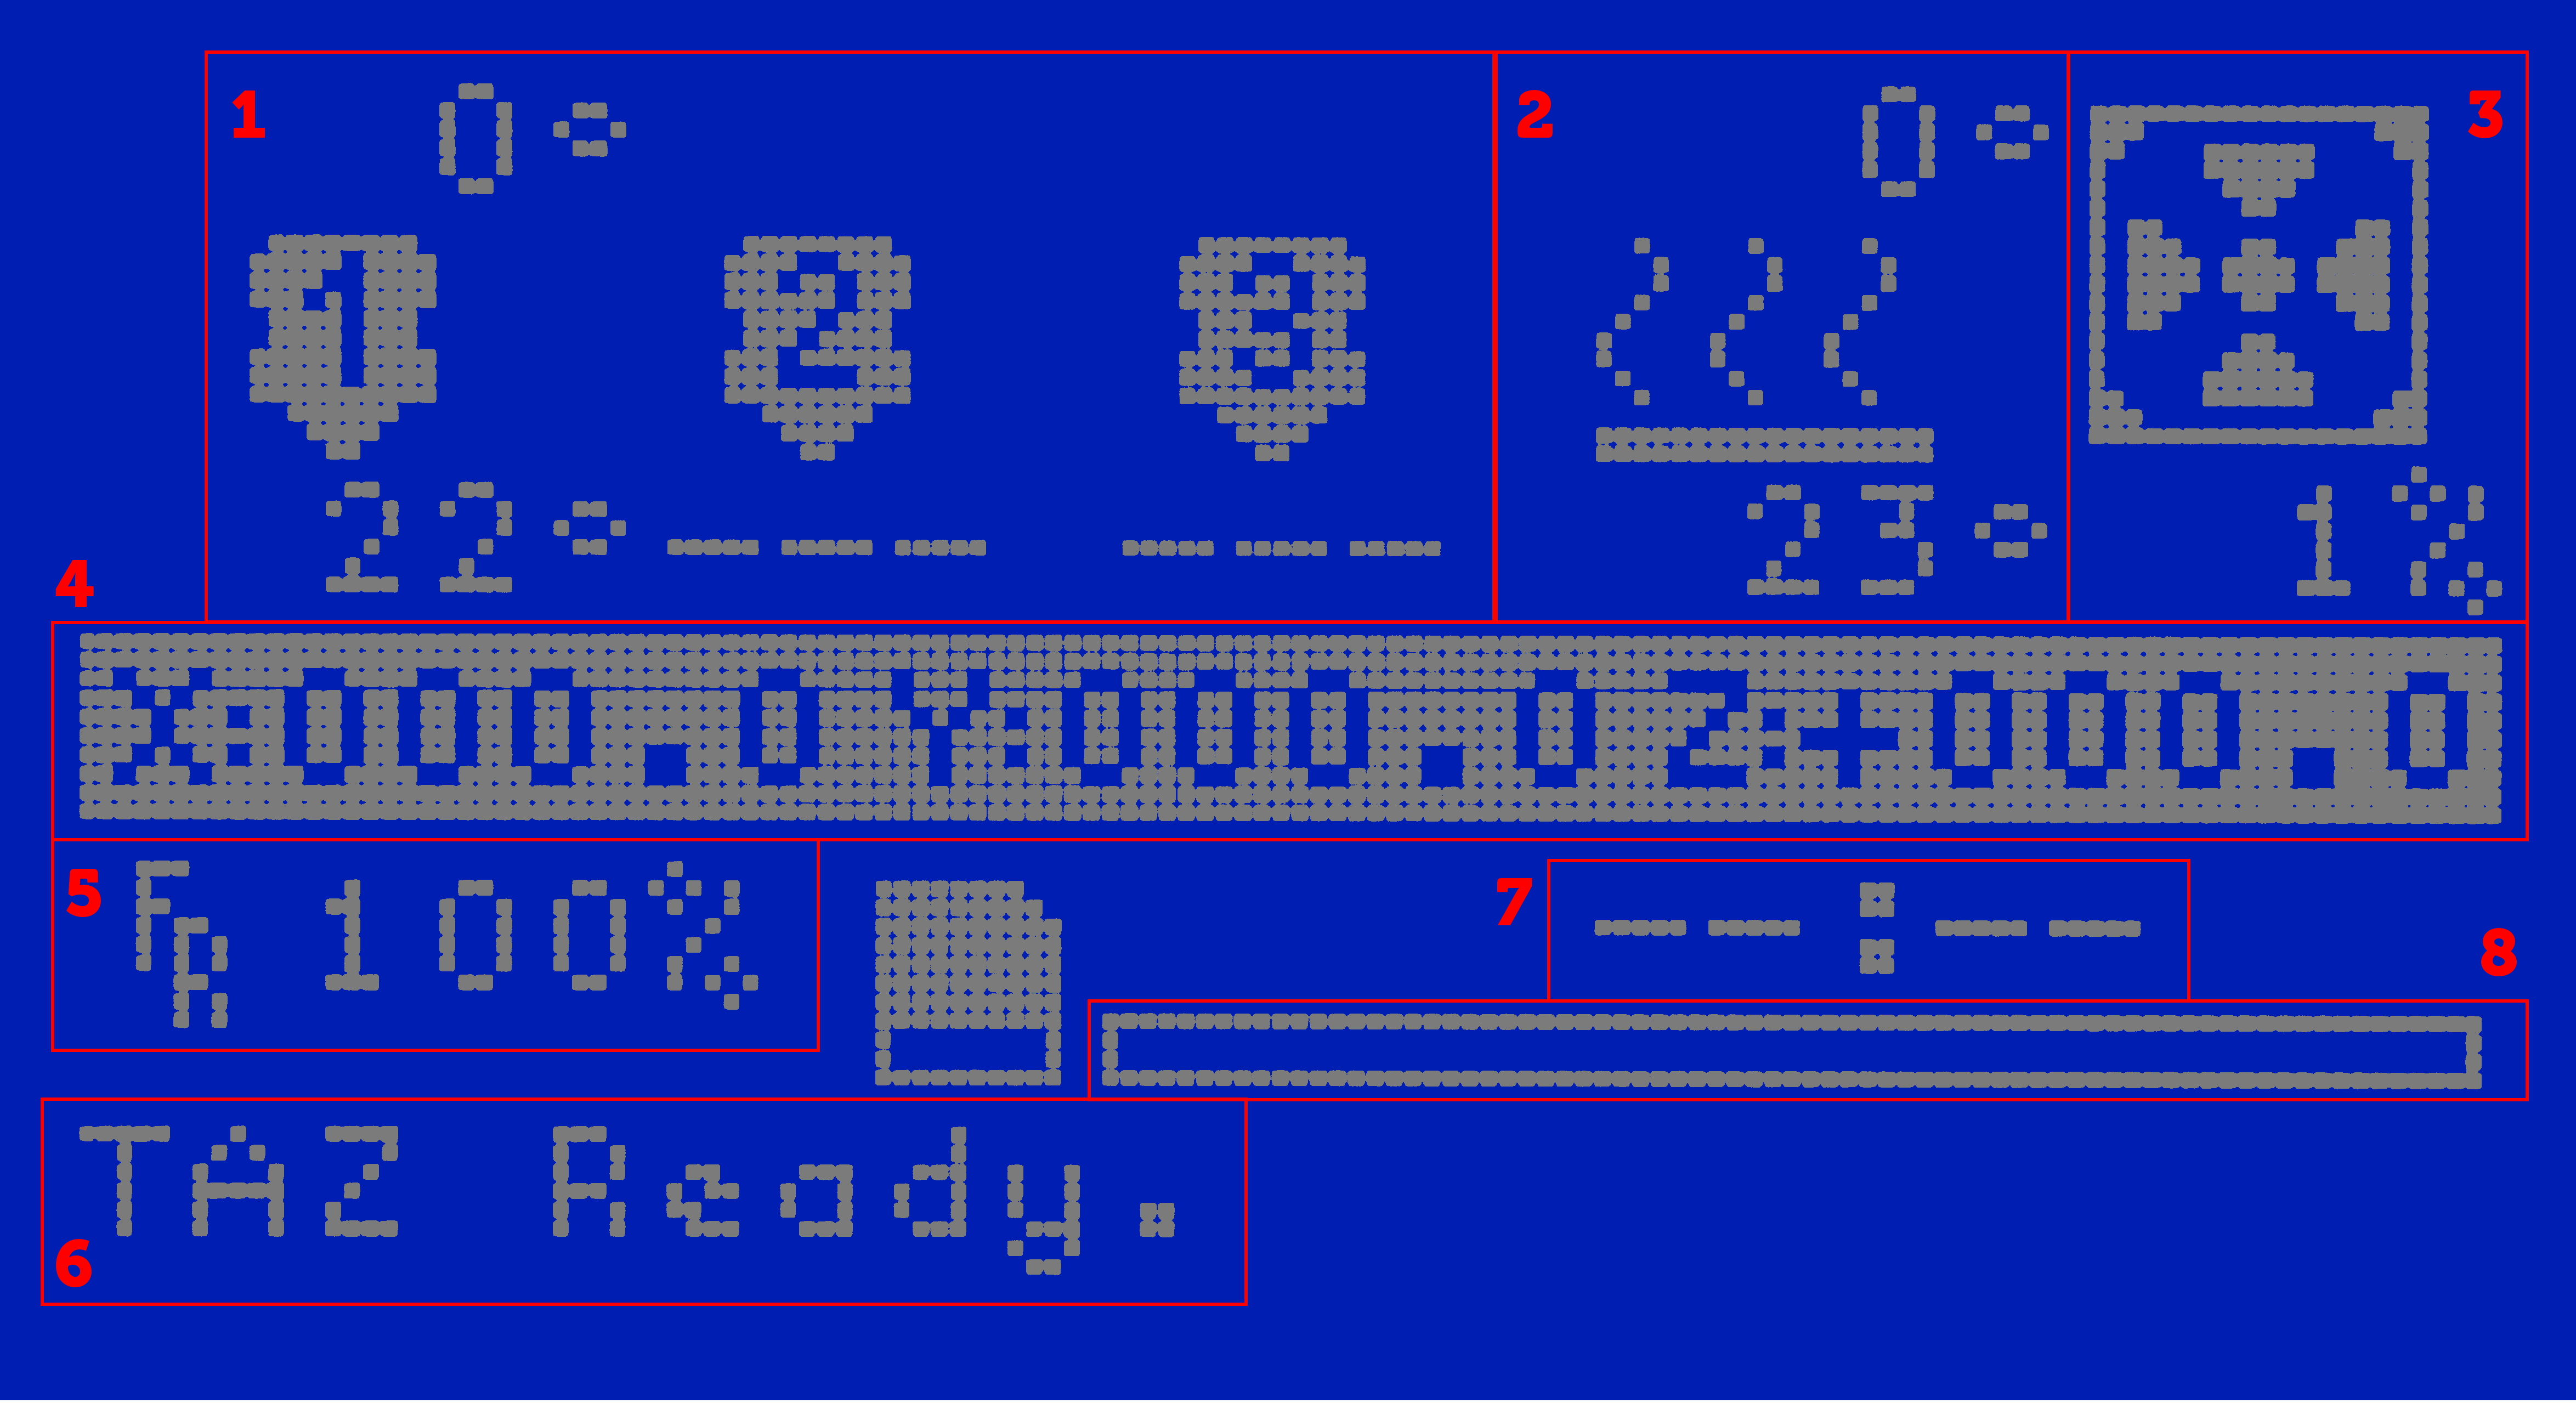
\includegraphics[keepaspectratio=true,angle=0,height=0.4\textheight,width=1.0\textwidth]{GLCD/info_screen_numbered.JPG}
\caption{GLCD Info Screen}
\label{fig:info_screen}
\end{figure}

\subsection{The Graphic LCD Status Screen}
After powering up your TAZ 3d printer the GLCD screen will turn on. After the start up screen you will see the Status screen (fig. \ref{fig:info_screen}, page \pageref{fig:info_screen}). The Status screen is the default screen for the GLCD, presenting the current status of the printer. There are a number of live statuses shown on the Status screen that will give you current temperatures, tool head coordinates, print status, and more. Shown in figure \ref{fig:info_screen} above are the different numbered sections of the status screen. Follow the key below for more information on each section.

\begin{enumerate}
\item Hot end temperatures: represents the current temperature (bottom) and set temperature (top) of up to three nozzles.
\item Heat bed temperature: represents the current temperature (bottom) and set temperature (top) of the heat bed.
\item Fan speed: represents the current fan speed. The fan is set to off (1\%) by default as this function is not used by the TAZ printer. If you later modify your TAZ printer to use a print cooling fan, this status indicator will come in use.
\item Tool head coordinates: represents the current tool head coordinates on the X, Y, and Z axes.
\item Feed rate: represents the current feed rate setting. The feed rate is set to 100\% by default which matches the speed set in the gcode generation. When on the status screen selection knob can be turned to increase or decrease the feed rate during the print. Increasing/decreasing the feed rate will increase/decrease the speed of the print.
\item Printer status: lists the current status of the printer including: SD card status, current printing file, or completed print time.
\item Current print time: lists the length of time for the current print job.
\item Progress bar: represents the progress of the current print job. When the bar is completely white the print is finished.
\end{enumerate}


\subsection{Using the Selection Knob}
To navigate through the LCD menu use the selection knob by rotating to scroll through selections and pressing the knob to make a selection. From the main status screen, press the knob to move into the menu screen (fig. \ref{fig:main_menu}, page \pageref{fig:main_menu}). To move backwards in the menu tree, select the top most menu selection on the current screen. Selections that will move you backwards through the menu tree are noted by an upwards facing arrow. Note that if the menu is left idle it will automatically move back to the main status screen.

\begin{figure}[h]
\centering
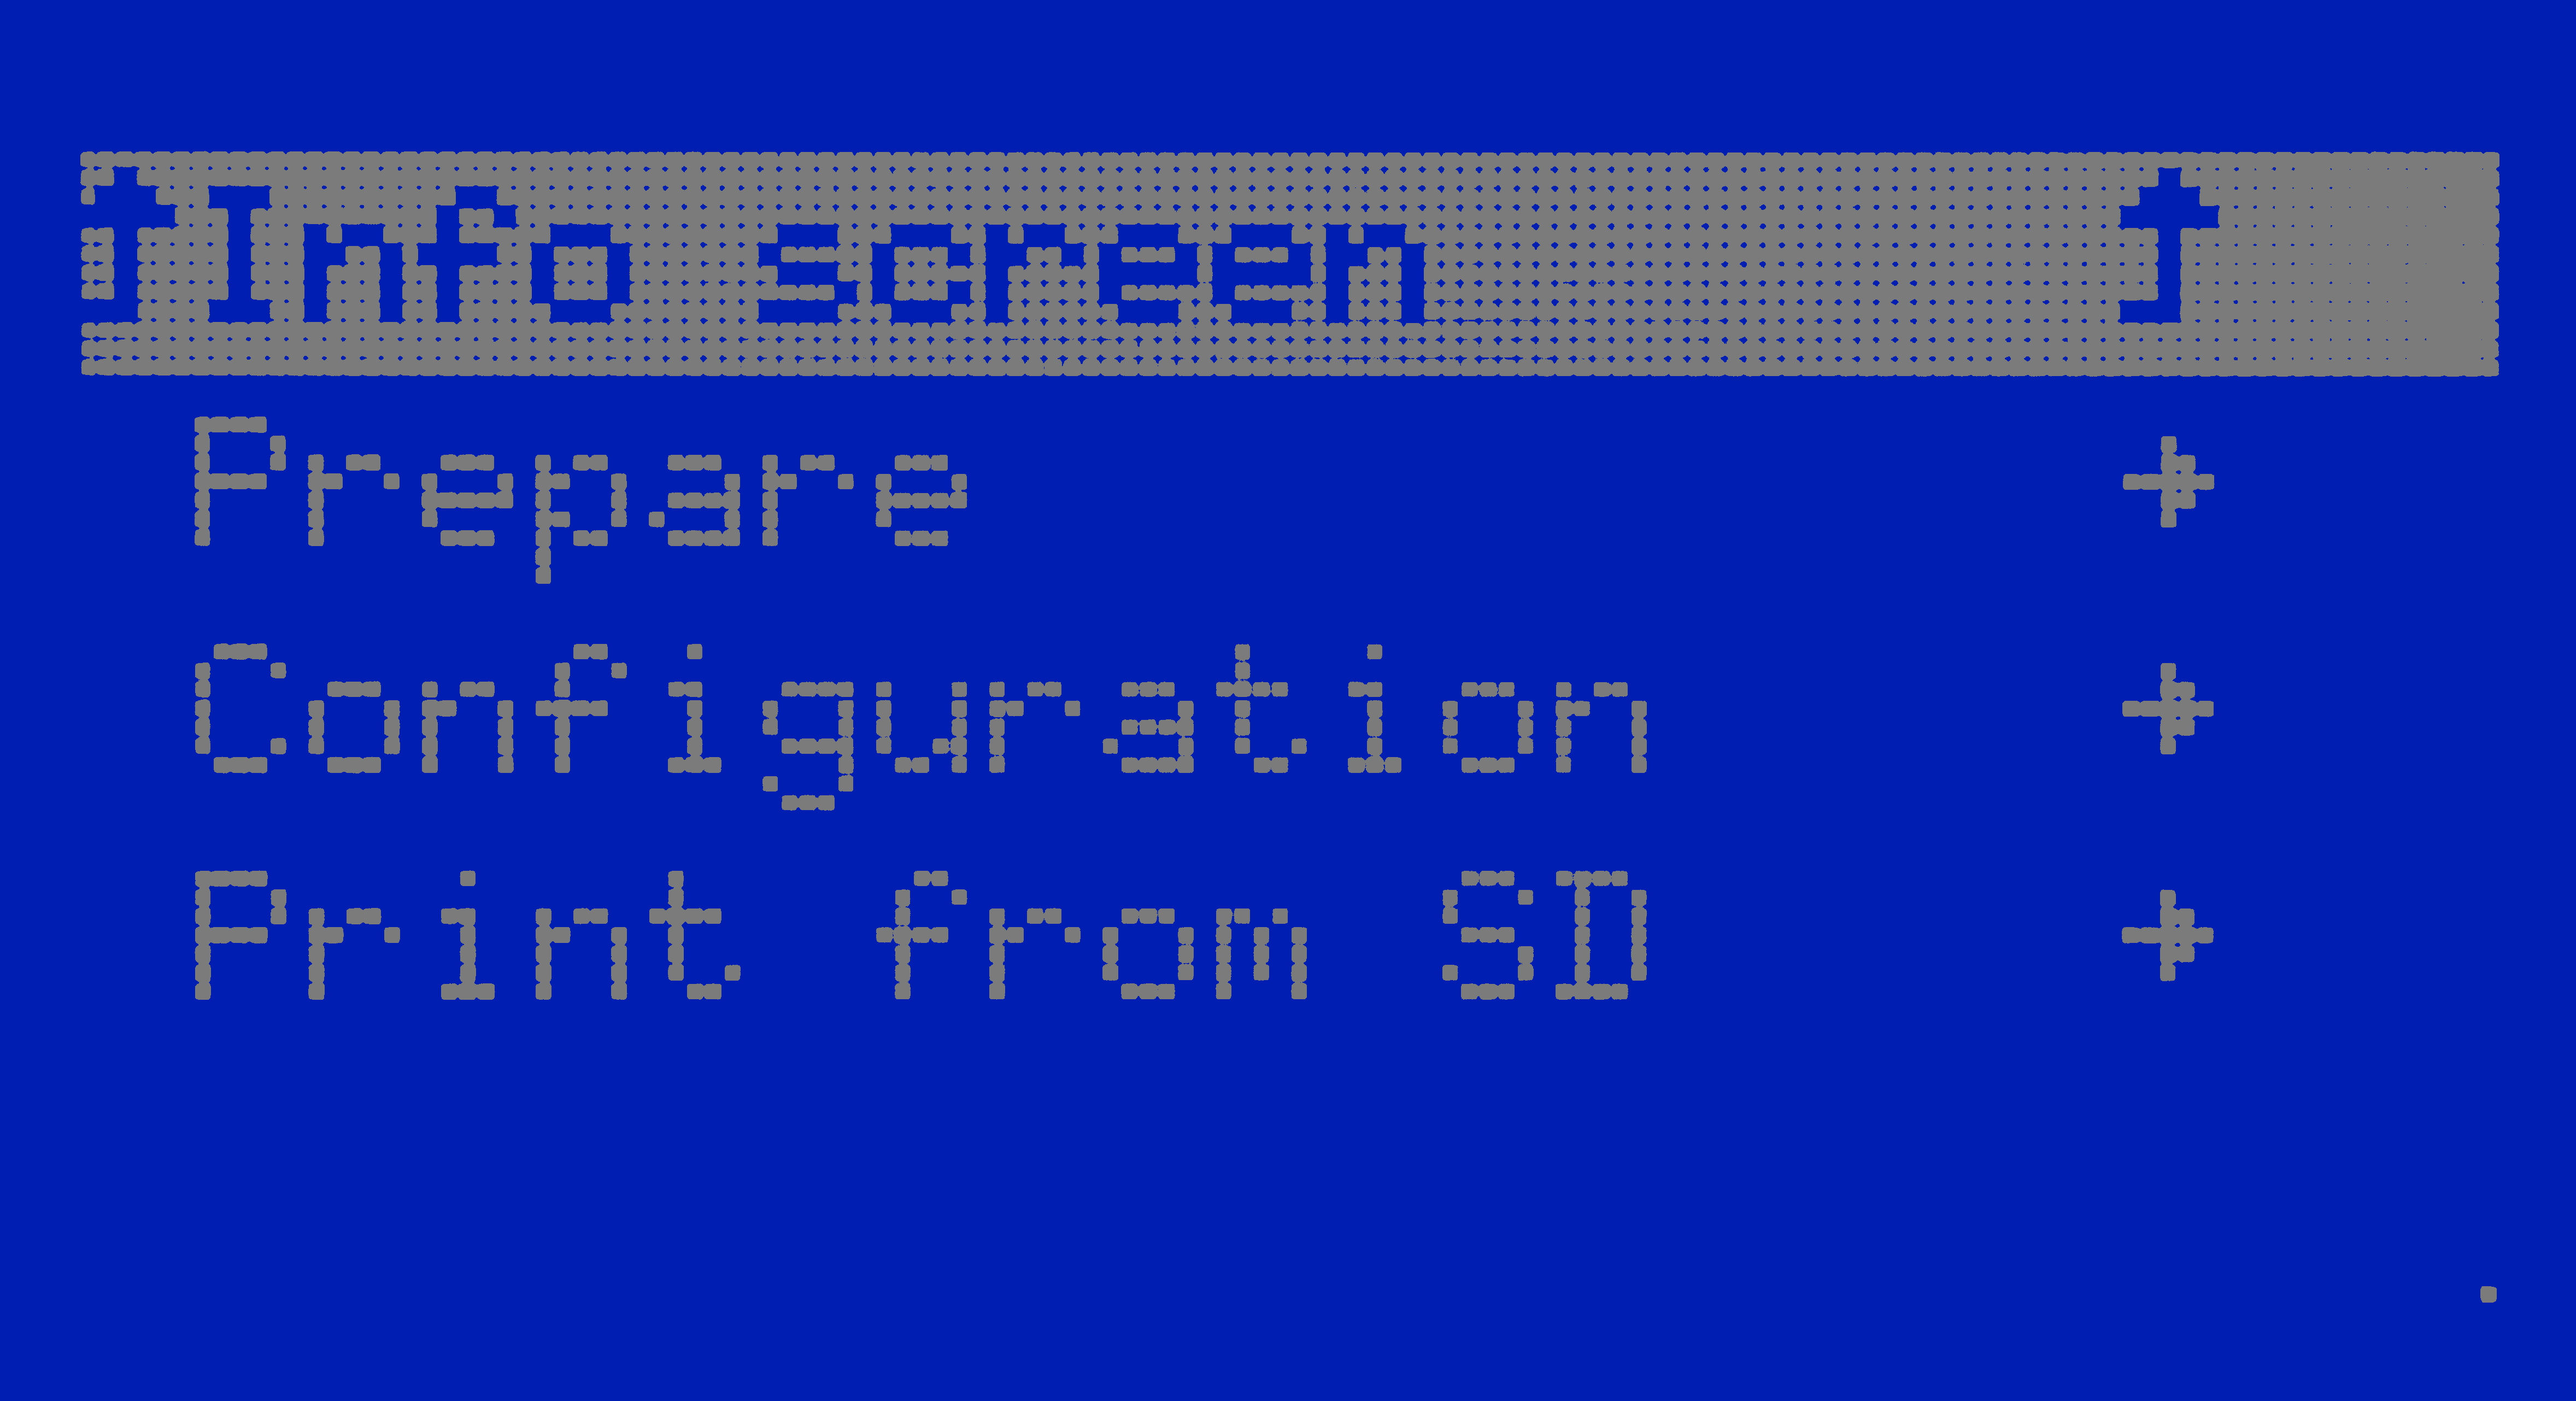
\includegraphics[keepaspectratio=true,angle=0,height=0.4\textheight,width=1.0\textwidth]{GLCD/main_menu.JPG}
\caption{Main menu}
\label{fig:main_menu}
\end{figure}

\subsection{Preparing for a Print}
Before starting a print you will need to set the hot end and heat bed to the appropriate temperatures for the filament type you are using. To quickly set the printer to preheat, for ABS or PLA filament, click the selection knob to bring up the menu and select \texttt{Prepare}. Select \texttt{Preheat PLA} for PLA filament or \texttt{Preheat ABS} for ABS filament. This will set the temperatures for the hot end and heat bed and begin bringing the printer up to print-ready temperature.

If you need to set the extrusion and/or bed temperature to a different setting than the preheat temperature you can manually set the temperature. To do so, from the main menu navigate through: Configuration \texttt{->} Temperature \texttt{->} Nozzle or Bed. Clicking on either of these settings will give you a menu to set and select the desired temperature setting.

\subsection{Selecting a File From the SD and Starting a Print}
Once the hot end and heat bed have reached the desired temperature the printer is ready to print. From the main menu select the \texttt{Print from SD} option. You will now see a selection of the directories and .gcode files on the SD card. Navigate through the menu to locate the file you would like to print. Select the desired file to begin the print.

\subsection{Making Manual Movements With the Graphic LCD}
As noted previously (page \pageref{sec:Graphic LCD or Printrun Host?}), making numerous manual movements is easier done using the Printrun host software. However, you can make manual movements with the GLCD. Navigate to Prepare \texttt{->} Move Axis. You will then select the length of the movement and then the axis to move. Note, that only 1mm and 0.1mm movements are allowed for the Z axis and extruder.

When at the move screen turn the selection knob clockwise to move the axis in millimeters in the positive direction and counter-clockwise for the negative direction. Push the selection knob to complete the manual move.

\subsection{Configuration Settings}

\begin{figure}[H]
\centering
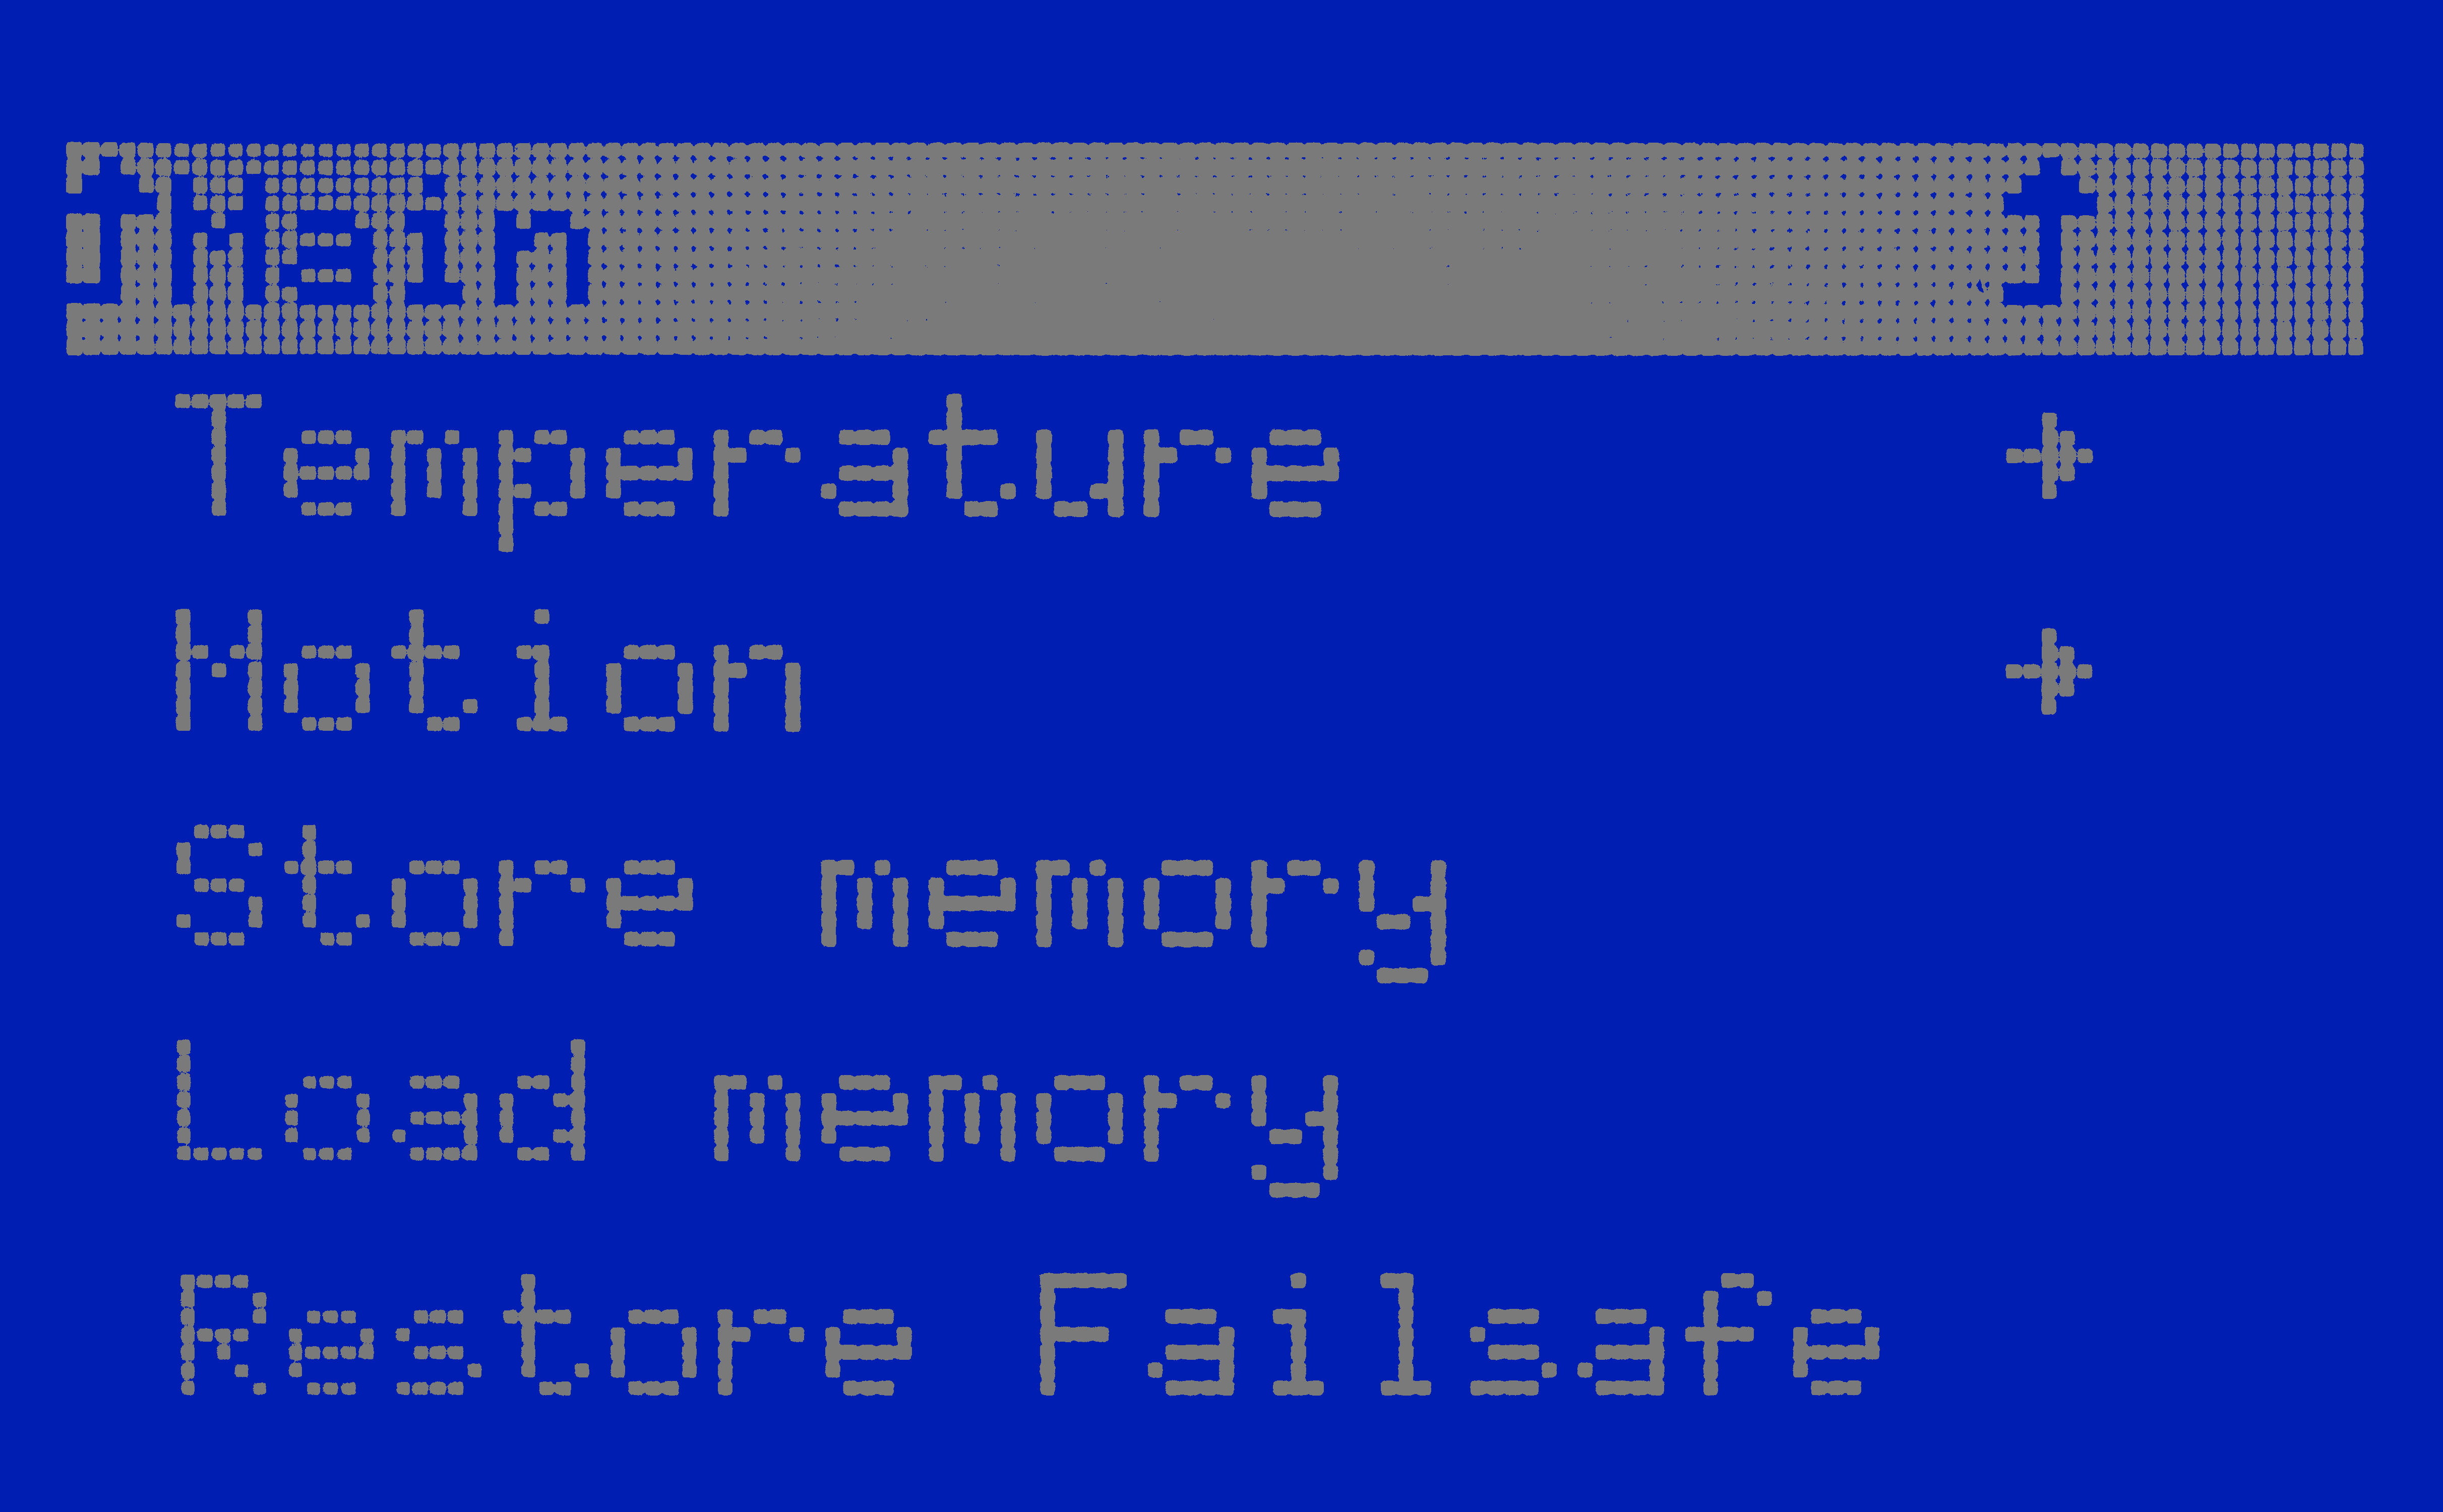
\includegraphics[keepaspectratio=true,angle=0,height=0.4\textheight,width=1.0\textwidth]{GLCD/configuration_menu.JPG}
\caption{Configuration Menu}
\label{fig:configuration_menu}
\end{figure}

Out of the box, the TAZ 3D printer is already calibrated for printing. However, the GLCD does allow tuning of the more advanced configuration settings. It is highly suggested to not modify the configuration settings unless you are certain it is needed.

To find the configuration settings, navigate to the main menu and then Configuration (fig. \ref{fig:configuration_menu}, page \pageref{fig:configuration_menu}). In the configuration settings you will find temperature and motion settings. These settings include default temperature settings, axis steps per mm, and more.

The \texttt{Store Memory} and \texttt{Load Memory} functions will store and load the changes you make using the GLCD Controller. You must use the \texttt{Store Memory} function to save the adjusted settings when the printer is powered down. The stored settings will then automatically load when the printer is repowered. If you ever need to revert back to the factory settings navigate to Configuration \texttt{->} Restore Failsafe. Clicking Restore Failsafe with set all configuration settings back to the original factory settings in the firmware.

For more information on the configuration settings please see the TAZ support page on LulzBot.com.

\subsection{GLCD Controller Menu Diagram}
\begin{figure}[H]
\centering
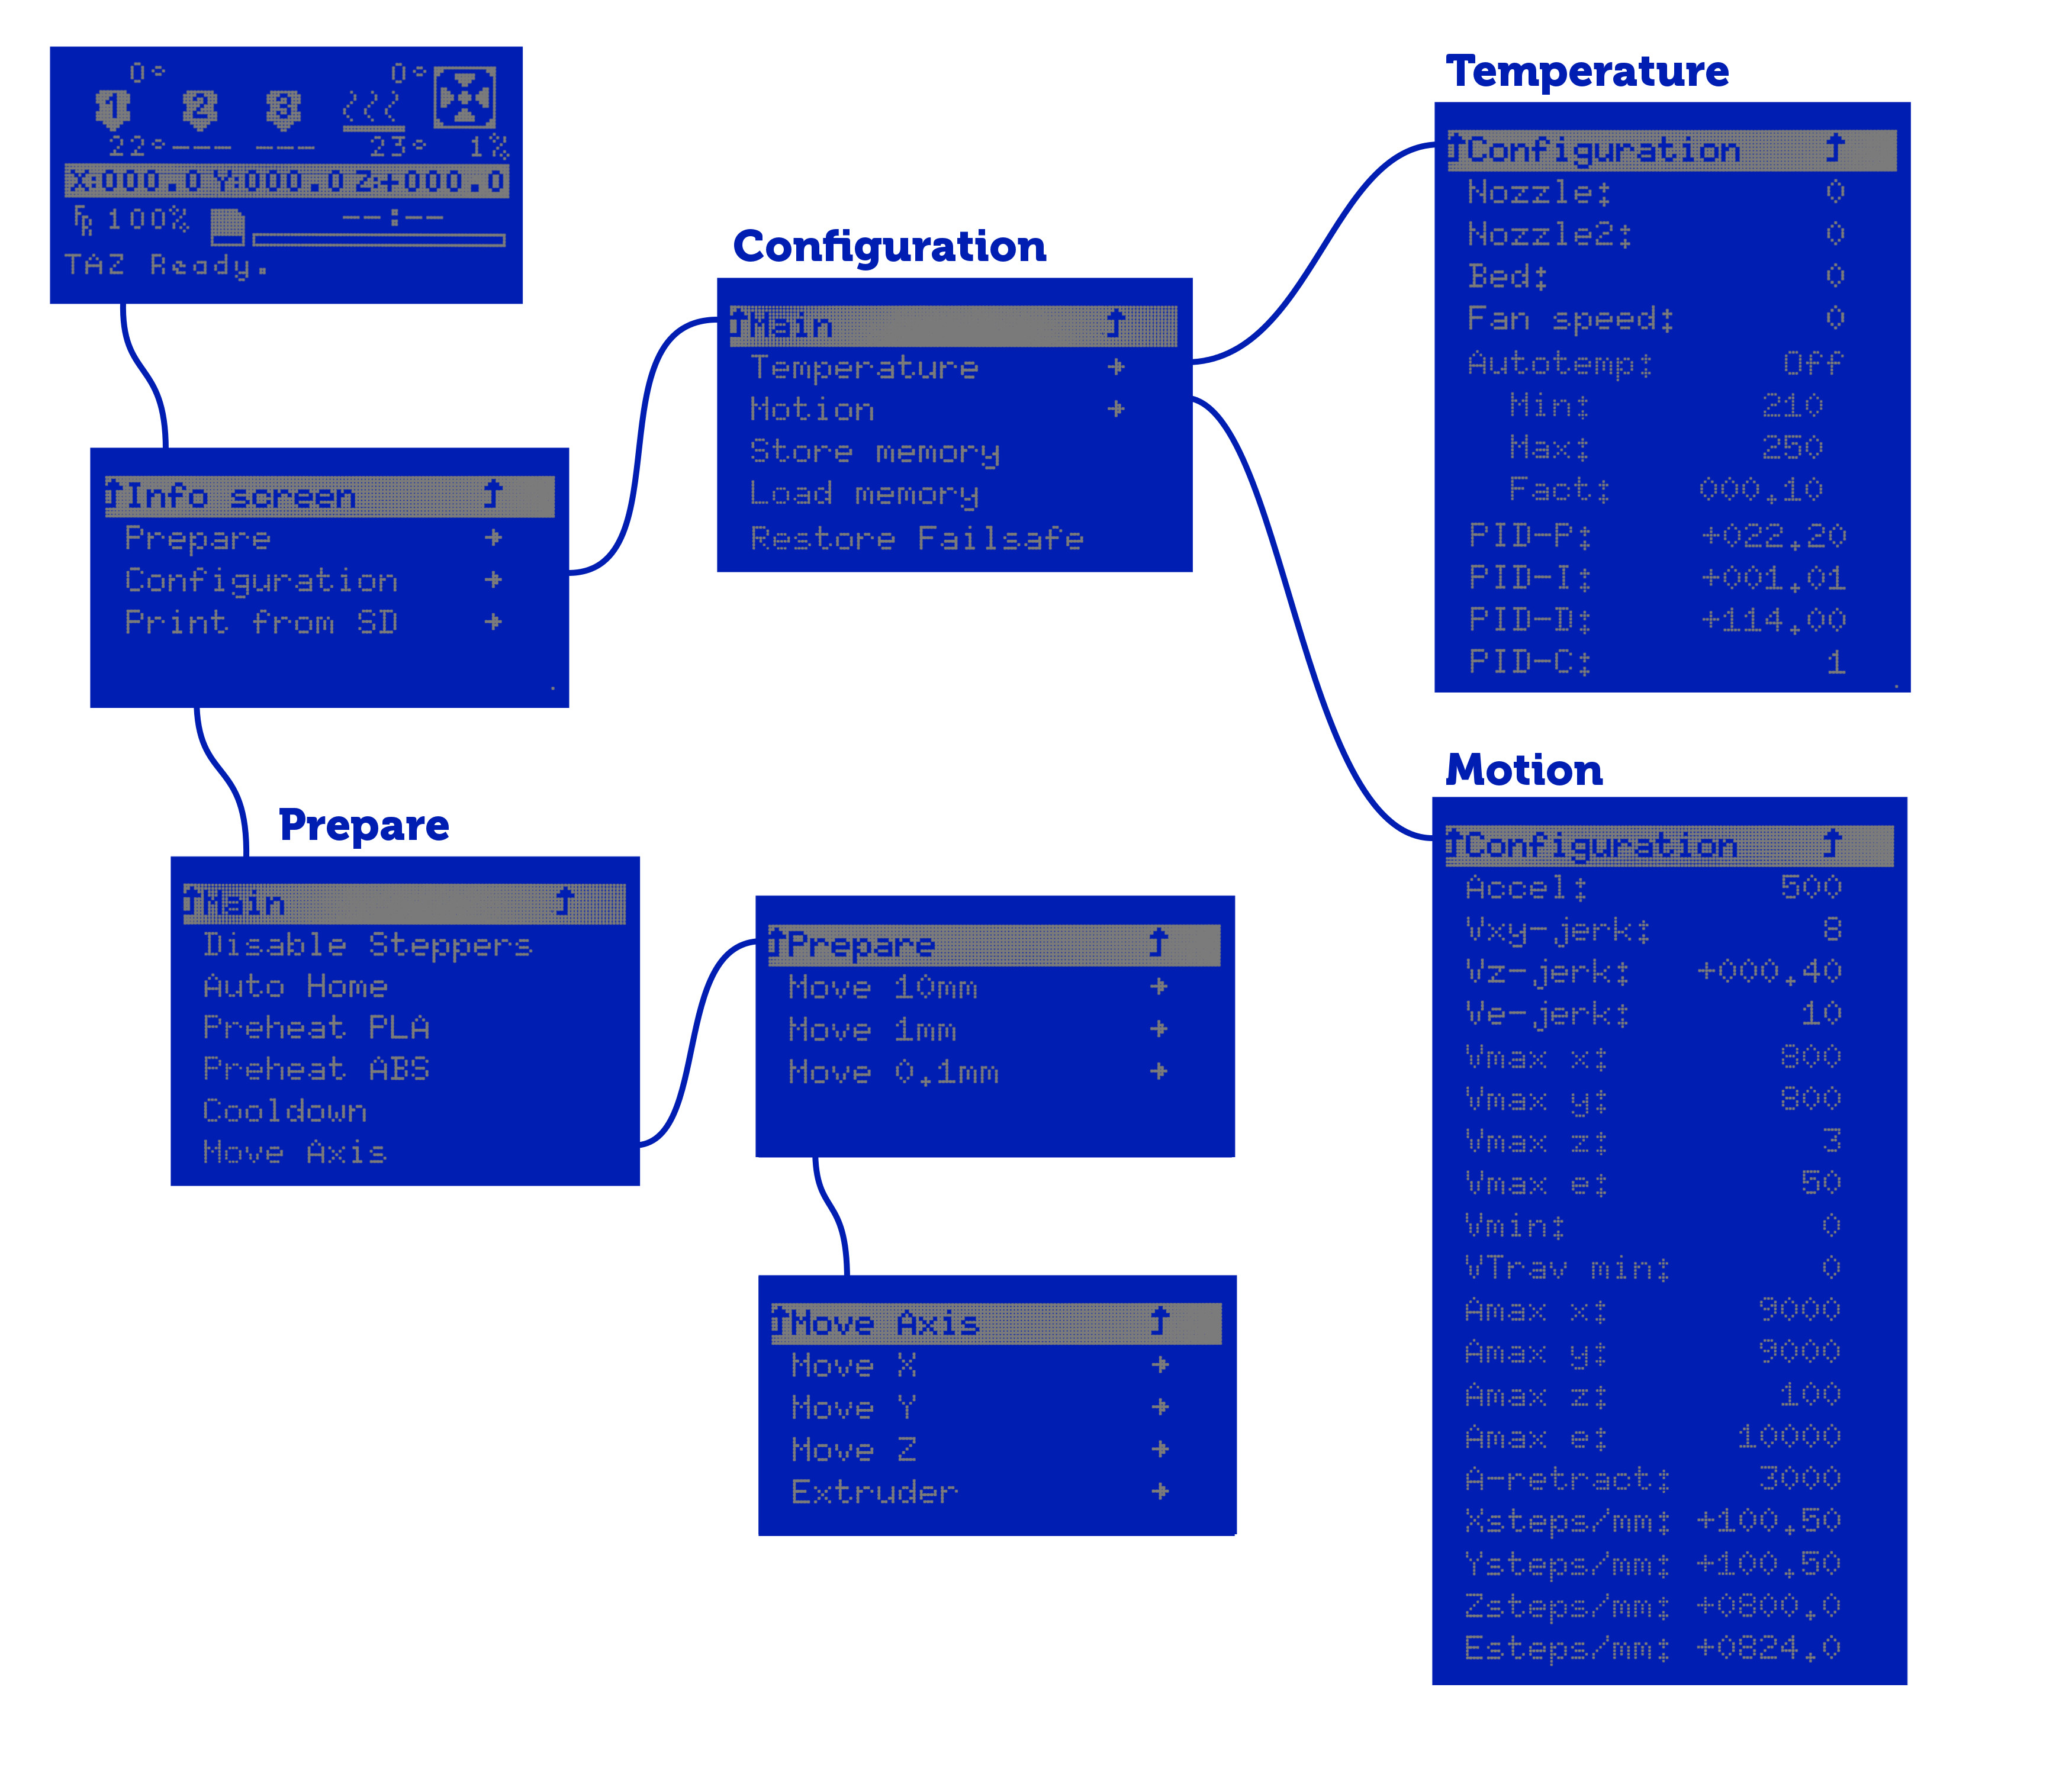
\includegraphics[keepaspectratio=true,angle=0,height=1.0\textheight,width=1.0\textwidth]{GLCD/glcd_menu.JPG}
\caption{Configuration Menu}
\label{fig:configuration_menu}
\end{figure}




